\documentclass[a4paper, 11pt]{article}

\usepackage{geometry}
\geometry{a4paper,left=30mm,right=30mm, top=35mm, bottom=30mm}

\usepackage[ngerman]{babel}
\usepackage[utf8]{inputenc} 
\usepackage[T1]{fontenc}
\usepackage{algorithm}
\usepackage{amsmath}
\usepackage{amssymb}
\usepackage{amsthm}
\usepackage{enumerate}
\usepackage{array}
\usepackage{wasysym}
\usepackage{fancyhdr}
\usepackage{graphicx}
\usepackage{hyperref}
\usepackage{tabularx}
\usepackage {tikz}
\usetikzlibrary {positioning}
%\usepackage {xcolor}
\definecolor {processblue}{cmyk}{0.96,0,0,0}
\usepackage{latexsym}
\usepackage{lastpage} % Seitenzahlen
%\usepackage{MNsymbol}
\pagestyle{fancy}
\usepackage[noend]{algpseudocode}
\usepackage{caption}
\usepackage{amsmath}
\usepackage{tikz}
\usetikzlibrary{arrows}
\usepackage{tabularx} %schöne tabellen
\parindent0pt %einrücken verhindern
\bibliographystyle{unsrt}

\usepackage{polynom}
\cfoot{\thepage  \ / \pageref{LastPage}}

% % % % % % % % % % % % % % % % % % % % % % % %
% % % % % % % % % % % % % % % % % % % % % % % %
\newcommand{\modullang}{BAs}
\newcommand{\semester}{SoSe 2018}
\newcommand{\modul}{BA}
\newcommand{\blatt}{}
\newcommand{\tutorium}{Mi 16-18 Uhr}
\newcommand{\tutor}{}
\newcommand{\datum}{\today}
\renewcommand{\proofname}{Proof}
% % % % % % % % % % % % % % % % % % % % % % % %
% % % % % % % % % % % % % % % % % % % % % % % %

\begin{document} 
	
	%%% Kopfzeile linker Bereich
	%      gerade Seite   ungerade Seite
	\rhead[ \leftmark   ]{\textbf{}}
	%%% Kopfzeile mittlerer Bereich
	%      gerade Seite   ungerade Seite
	\chead[\leftmark   ]{\leftmark{}}
	%%% Kopfzeile linker Bereich
	%      gerade Seite             ungerade Seite
	\lhead[\textbf{}]{\blatt}
	
	
	%-- Deckblatt --						      
	\thispagestyle{empty}
	\begin{center}
		
		\vspace*{1.4cm}
		{\LARGE \textbf{Technische Universität Berlin}}
		
		\vspace{0.5cm}
		
		{\large Notes\\[1mm]}

		
		
		\vspace{1.0cm}
		{\LARGE \textbf{BlUB}}\\
		\vspace*{1.0cm}
		
		
		%	Babak \\
		%	Frank \\
		%	Kristian \\
		%	Rodrigo \\
		Sascha Lange%, 349960
		
		
		
	\end{center}
	
	\renewcommand{\labelenumi}{\alph{enumi})}
	\renewcommand{\labelenumii}{(\roman{enumii})}
	\renewcommand{\labelenumiii}{\arabic{enumiii}.}
	\renewcommand{\contentsname}{Table of Contents}
	%\renewcommand{\labelenumii}{\textbf{-}}	
	%-- Eigentlicher Text --
	\newpage
	\newtheorem{Cor}{Corollary}
	\newtheorem{Theorem}{Theorem}
	\newtheorem{Def}{Definition}
	\newtheorem{Prop}{Proposition}
	\newtheorem{Lemma}{Lemma}
	\section*{Meta Blub}
	
	Let $\mathcal{S}$ denote state space and $\mathcal{A}$ denote action space. Let $\mathcal{P}=\{1,...,P\}$ be  the set of players and $\mathcal{N}=\{N_0,...,N_{P}\}$ the set of (neural network) function approximators, where $N_i : \mathcal{S} \mapsto \mathcal{A}$, $N_i(s) = a$, %$s\in\mathcal{S}, a\in\mathcal{A}$,
	corresponds to player $i$. \\
	
	\begin{Def}[Agreement, stability] {Let $i\in\mathcal{P}, s, s'\in\mathcal{S}$.}
		\begin{itemize}
%			\item[i)] Player $i$ agrees on two states $s, s'$, if $N_i(s) = N_i(s')$
			\item[i)] Agreement between two states $s,s'$ is defined as the ratio  $\frac{1}{P}\cdot|\{ i \in\mathcal{P}: N_i(s) = N_i(s')\}|$
%			\item[ii)] Players $i, j$ agree on one state $s$, if $N_i(s) = N_j(s)$
			\item[ii)] Stability of a state $s$ is defined as the ratio
			$\frac{2}{P(P-1)}\cdot|\{ (N_i, N_j) \in\mathcal{N}\times\mathcal{N}: N_i(s) = N_j(s), i\neq j\}|$
		\end{itemize}
		
	\end{Def}

	Then we can define
	\begin{Def}[Distance] {Let $i\in\mathcal{P}, s, s'\in\mathcal{S}$.}
		\begin{itemize}
			\item[]  The distance d between two states is given by: $d(s, s') = 1 - Agreement(s,s')$
		\end{itemize}
		
	\end{Def}
	After having observed data $D = \{(s_1, a_1),...,(s_n,a_n)\}$ from a new teammate $p$, we can give the action classifier as 
	\begin{align*}
	C_p(s) = \underset{a}{argmin} \{ d(\tilde{s}, s): (\tilde{s}, a)\in D \}
	\end{align*}
	
	The goal is, to combine the two notions in Definition 1, to obtain a $similarity$ of two states, relative to our teammate (for reasons I explained on slack). What I initially suggested was to do it manually (i.e. no NN training), however, I think this can be done using meta learning in the following way: \\

	
	Let $C_{\theta}$ denote our meta classifier. We want to learn $\theta=\theta_0$, such that
	\begin{itemize}
		\item after small number L of gradient steps on data $D$ from agent $A$, to obtain $\theta_L$, the network $C_{\theta_L}$ performs well on predicting actions of $A$
	\end{itemize}
	So we obtain updated network params after $i\leq L$ steps on $D$ from $A$ by
	\begin{align*}
	\theta^A_i = \theta^A_{i-1} - \alpha \Delta_{\theta} \mathcal{L}_A(C_{\theta^A_{i-1}})
	\end{align*} for a \textbf{single} Task $A$, and thus the meta-objective becomes
	\begin{align*}
	\sum_{A \in POOL} \mathcal{L}_{P}(C^A_{\theta_L}) =: \mathcal{L}_{Meta}, 
	\end{align*} where $\mathcal{L}_{P}$ denotes the loss on the hold out set corresponding to $A$. Both $A$ and $P$ are agents, but $A$ denotes agents at training time and $P$ denotes agents at test time, indicating that players can be humans. Note however, that \textbf{the different notation simply denotes disjoint data, but from the same agent P=A}.
	
	Finally we have the outer loop update given by
	\begin{align*}
	\theta_0 = \theta_0 - \beta \Delta \mathcal{L}_{Meta}.
	\end{align*}
	
	Using the idea of incorporating implicit soft cluster assignment (see slack) into the learning process we may obtain for $C_\theta$ the following architecture:\\
	
	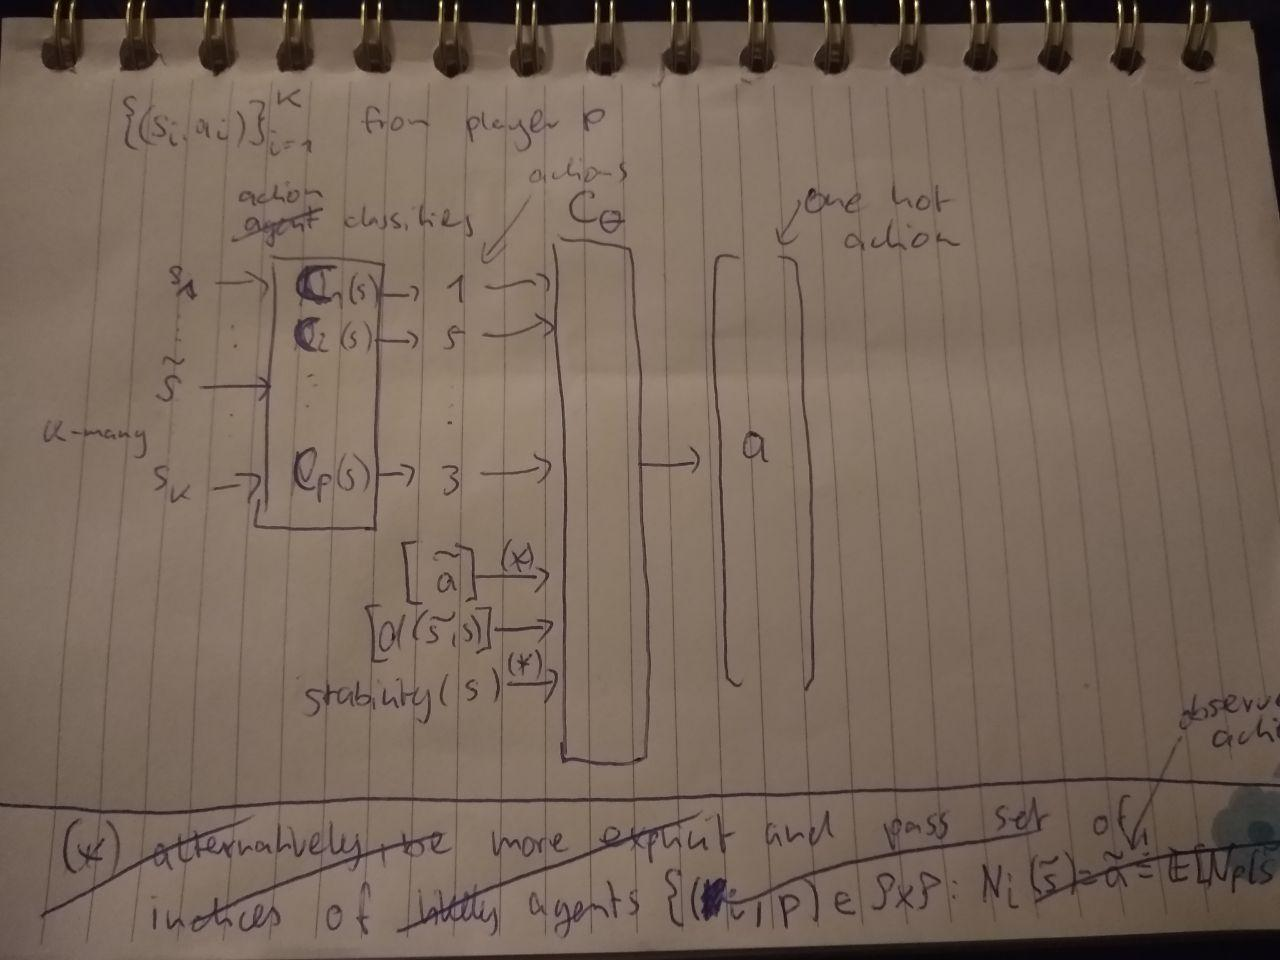
\includegraphics[scale=.5]{architecture}
	
	%When observing a new player $p$ and using the notion of stability of a state, we can try to estimate the relative skill of $p$, by computing $\frac{2}{P(P-1)}\cdot|\{ (N_i, p) \in\mathcal{N}\times\mathcal{N}: N_i(s) = E[N_p](s)\}=:D|$, where $E[N_p](s)$ will be observed through actual playing with $p$ and observing state action pairs $(s,a)$. Define the set of players $\bar{D} = \{ (N_i, p) \in\mathcal{N}\times\mathcal{N}: N_i(s) \neq E[N_p](s)\}$, for which a different action than $a$ has been predicted. The goal is, using meta-learning, to increase the weight of players in $D$ and decrease the weight of players in $\bar{D}$, to get a notion of similarity, that is relative to the player we want to predict actions for. \\
	%Let d(s, s') be given by the inverse $Agreement$ of $s$, and $s'$.
	%In order to be able to cast this into the MAML framework, we define the set of possibly infinite tasks to be set of possible teammates (for which we want to predict actions).
	%During training of the meta learner, we are trying to find out how to change for different possible teammates the weights (coming from $D$ and $\bar{D}$ each step) for similarity computation, such that predictions of actions using the ensemble of agent networks, will be most accurate.
	
	%Training:
	%will do this today
	
	
	
\end{document}

%Python’s default arguments are evaluated once when the function is defined, not each time the function is called (like it is in say, Ruby). This means that if you use a mutable default argument and mutate it, you will and have mutated that object for all future calls to the function as well. (https://docs.python-guide.org/writing/gotchas/)
